\documentclass[11pt]{article}
\usepackage{enumerate}
\usepackage{fancyhdr}
\usepackage{amsmath}
\usepackage{graphicx}

\thispagestyle{empty}
\setlength{\parindent}{0cm}
\setlength{\parskip}{0.3cm plus4mm minus3mm}
\oddsidemargin = 0.0in
\textwidth = 6.5 in
\textheight = 9 in
\headsep = 0in

\title{CSCI 4100 Fall 2018 \\
% enter assignment number
Assignment 10 Answers}
\author{Damin Xu\\661679187}


\begin{document}
\maketitle
% enter question #
\noindent{\bf Exercise 6.1}
\begin{enumerate} [(a)]
	\item \begin{enumerate} [1.]
		\item Two vectors with very high cosine similarity but very low Euclidean distance similarity:\\
		vector1: [1, 1], vector2: [1000, 1010],\\ Eucildean Distance: 1419.888, Cosine Similarity: 0.9999876
		\item Two vectors with very low cosine similarity but very high Euclidean distance similarity:\\
		vector1: [0.1, 0.1], vector2: [-0.1, -0.1],\\ Eucildean Distance: 0.2828, Cosine Similarity: -1
	\end{enumerate}
	\item When the origin changes, cosine similarity changes only a little bit, but Euclidean distance similarity keeps the same. This may not affect y choice of features.
\end{enumerate}


\noindent{\bf Exercise 6.2}
If f(x) $\geq \frac{1}{2}$ and $y = -1$,  
\[
\begin{aligned}
	e(f(x)) &= P[f(x)\neq y]\\
	&= P[f(x) = +1, y=-1]+P[f(x) = -1, y=+1]\\
	&= 1\times(1-\pi(x))+0\times\pi(x)\\
	&= 1-\pi(x)
\end{aligned}
\]
If f(x) $\leq \frac{1}{2}$ and $y = +1$, 
\[
\begin{aligned}
	e(f(x)) &= P[f(x)\neq y]\\
	&= P[f(x) = +1, y=-1]+P[f(x) = -1, y=+1]\\
	&= 0\times(1-\pi(x))+1\times\pi(x)\\
	&= \pi(x)
\end{aligned}
\]
Thus, $e(f(x)) < \pi(x)$ for $\pi(x) \geq \frac{1}{2}$, and $e(f(x)) < 1-\pi(x)$ for $\pi(x) \leq \frac{1}{2}$. So at any time, $e(f(x))=min(\pi(x),1-\pi(x))$, and this indicates $e(f(x))\leq\frac{1}{2}$. Therefore error of any other hypothesis function $e(h(x))\geq min(\pi(x), 1-\pi(x))$.
\newpage
\noindent{\bf Problem 6.1}
\begin{enumerate} [(a)]
	\item \ \begin{figure}[htb] 
			{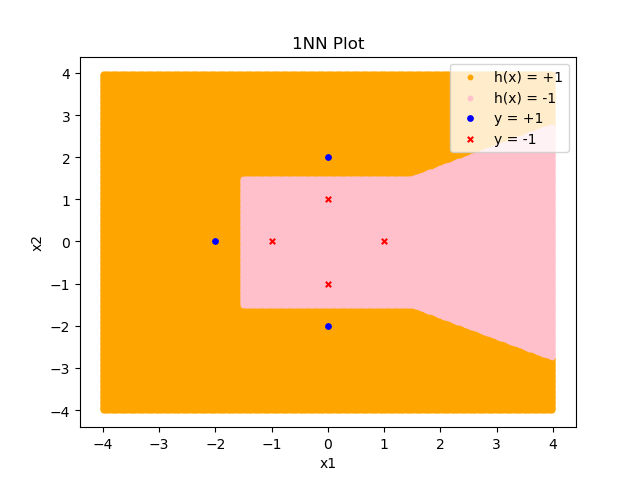
\includegraphics[height=8.5cm]{p6_1_a_1.png}}
	\end{figure}
	\begin{figure}[htb] 
			{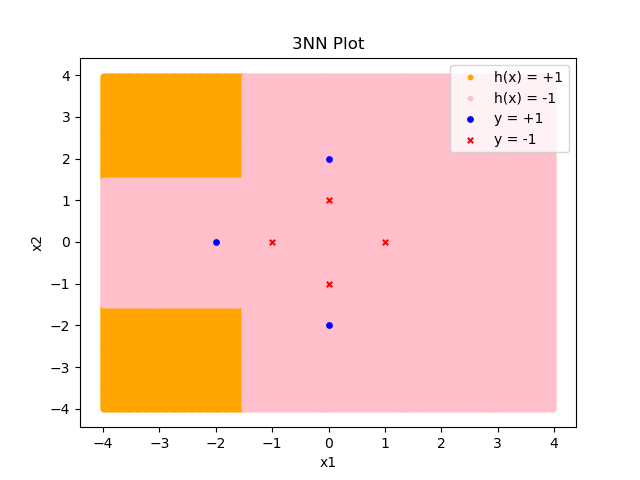
\includegraphics[height=8.5cm]{p6_1_a_3.png}}
	\end{figure}

	\newpage

	\item \  \begin{figure}[htb] 
			{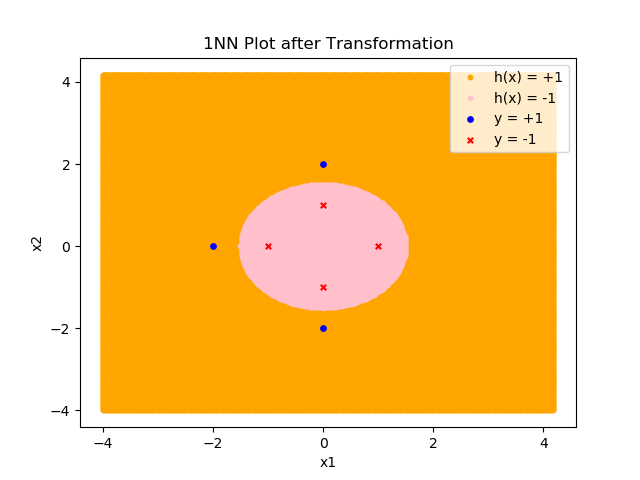
\includegraphics[height=8.5cm]{p6_1_b_1.png}}
	\end{figure}
	\begin{figure}[htb] 
			{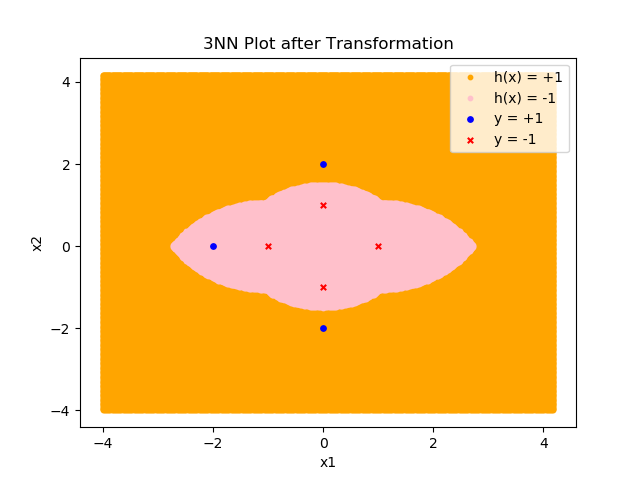
\includegraphics[height=8.5cm]{p6_1_b_3.png}}
	\end{figure}
\end{enumerate}

\newpage

\noindent{\bf Problem 6.4}
	\begin{figure}[htb] 
			{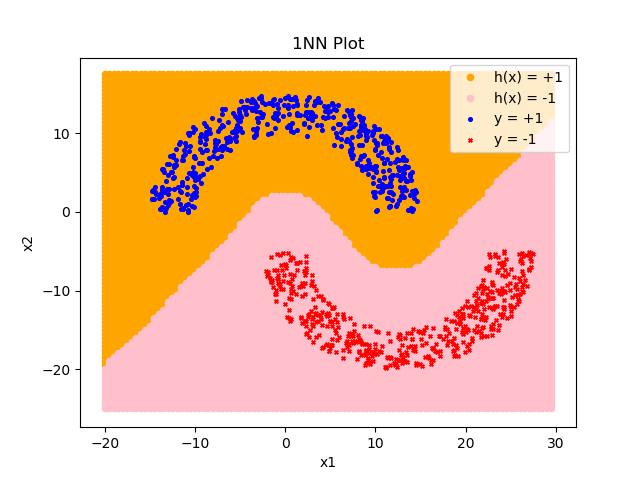
\includegraphics[height=8.5cm]{p6_4_1.png}}
	\end{figure}
	\begin{figure}[htb] 
			{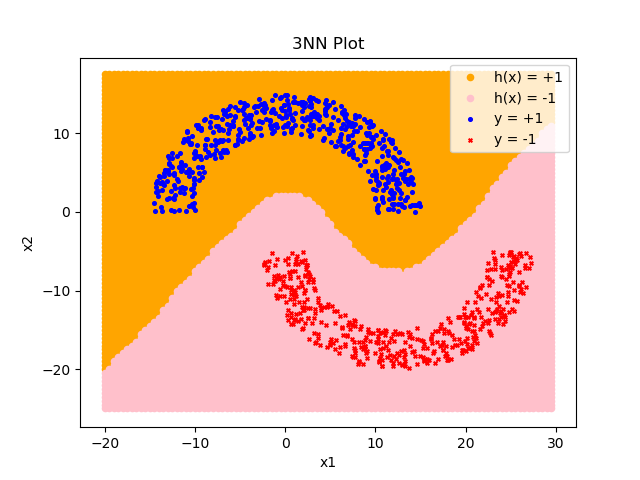
\includegraphics[height=8.5cm]{p6_4_3.png}}
	\end{figure}

\newpage

\noindent{\bf Problem 6.16}
\begin{enumerate} [(a)]
	\item Time cost for finding the nearest neighbor with partition: 20.435 seconds.\\
		Time cost for finding the nearest neighbor with brute force: 153.322 seconds.
	\item Time cost for finding the nearest neighbor with partition: 28.723 seconds.\\
		Time cost for finding the nearest neighbor with brute force: 158.261 seconds.
	\item Finding the nearest neighbor by using the partition with branch and bound cost much less time than the brute force approach, because the brute force approach go through all 10000 training point for every test point, whereas by using partition, for each point, only distances from about $\frac{1}{10}$ of points need to be compared with. Thus using partition shortens a lot of time.\\
	\\
	Also, Finding nearest neighbor using data of gaussians distributions will cost much more time than using uniform data when running partition algorithm. The reason is that for gaussians distribution, most points located in the center part of coordination, and huge amount of points located in a few regions, and remaining regions only have relativly a few points. So if the test point is located at the center regions, the program needs to go through a mountain of points to compare the distance. 

	\item Yes, because for small amount of data, partition have little effect on running time, and if the data set is small enough, the partition might cause even more time.
	
\end{enumerate}
\end{document}
\end{document}
